\documentclass{standalone}
\usepackage{tikz}
\usetikzlibrary{patterns, positioning}
\usepackage[sfdefault]{ClearSans} %% option 'sfdefault' activates Clear Sans as the default text font
\usepackage[T1]{fontenc}

\begin{document}
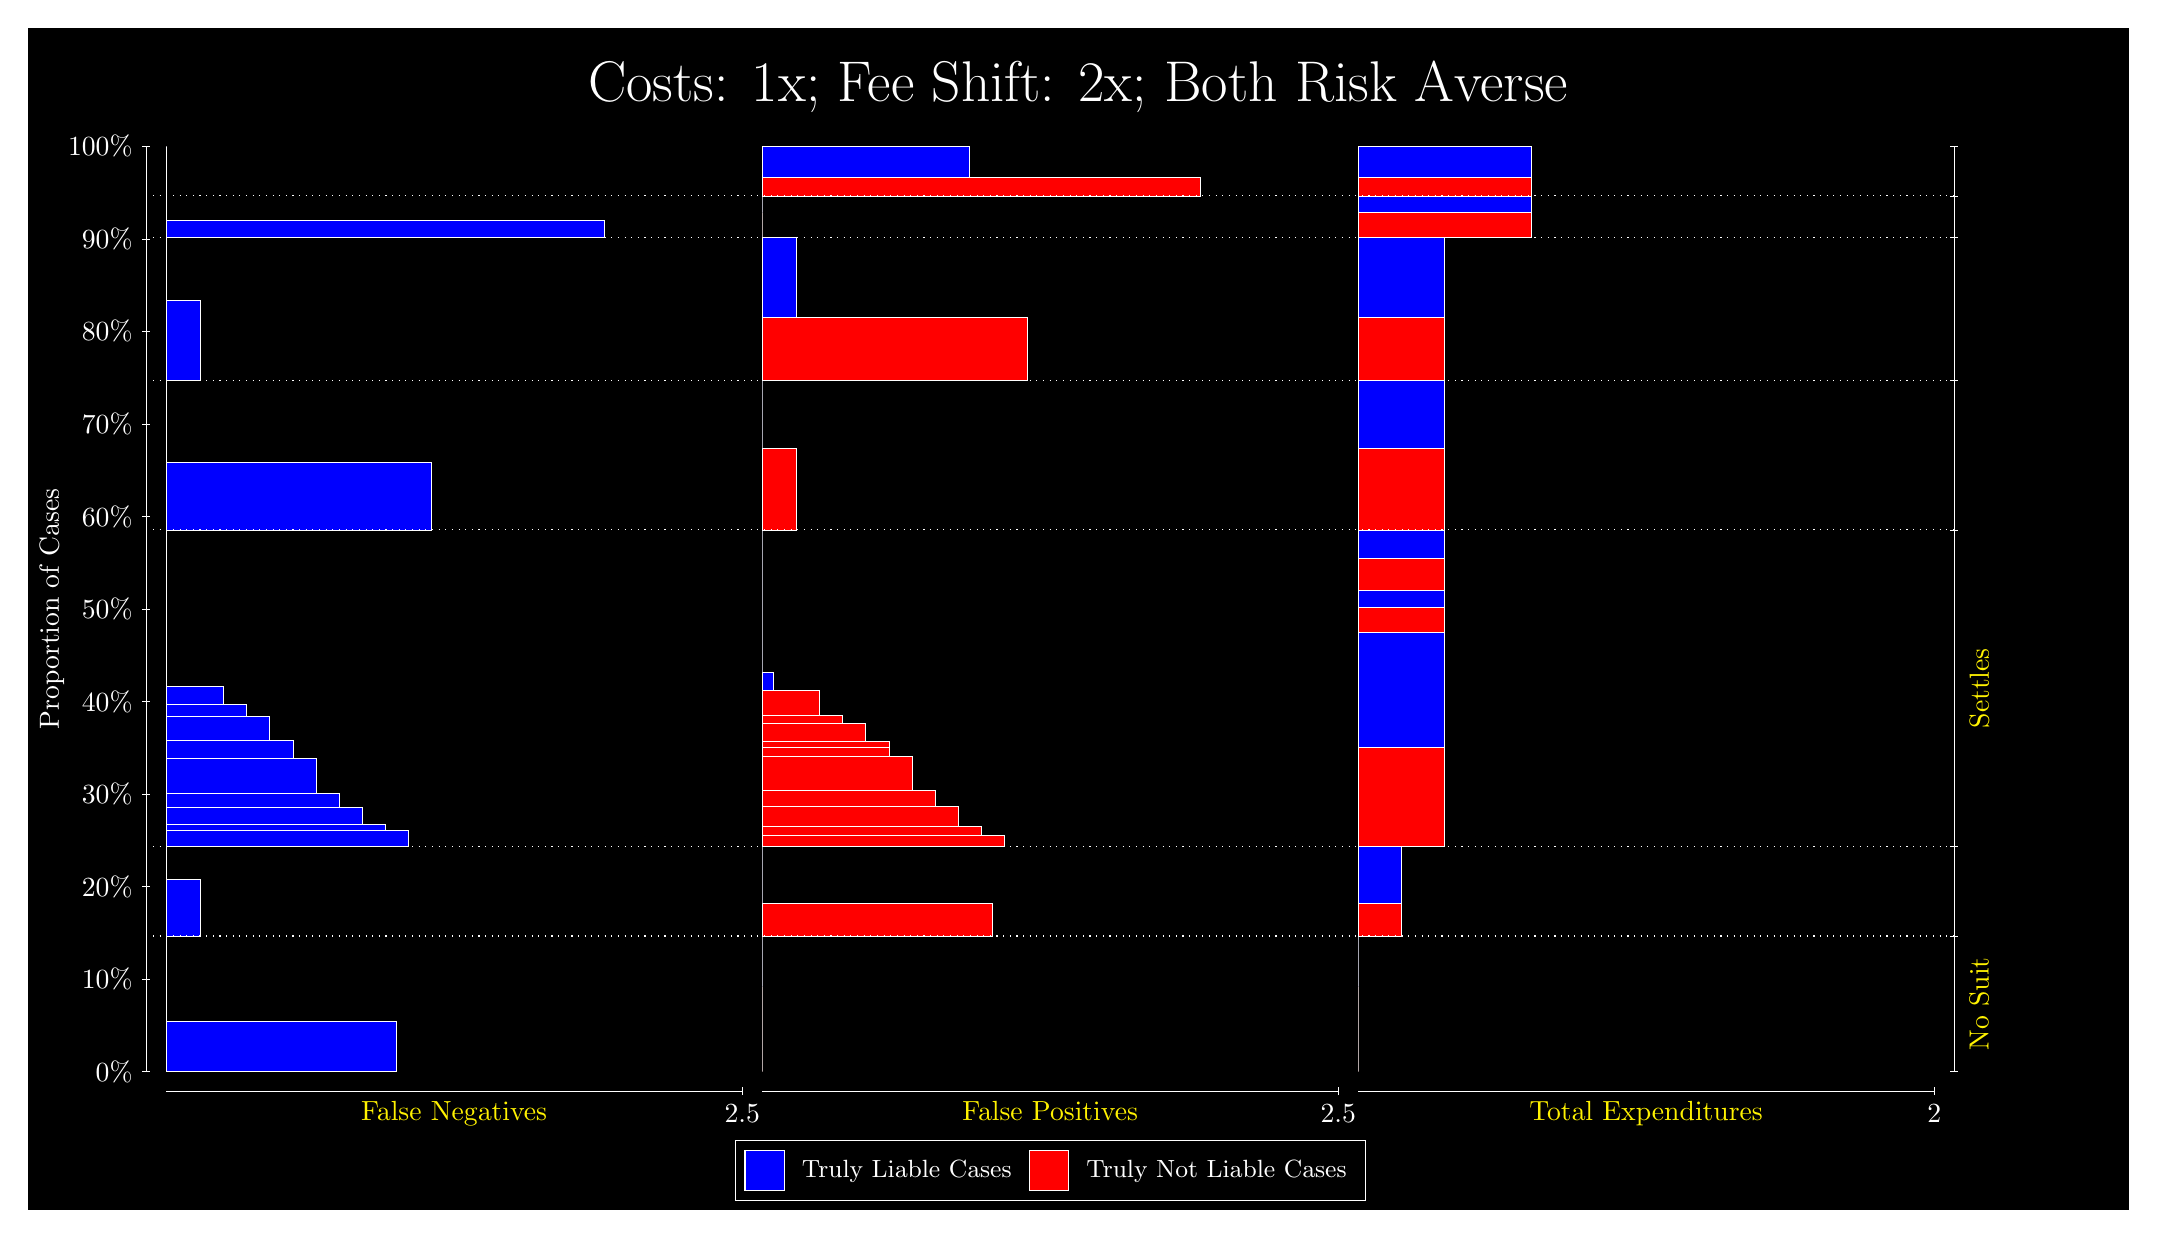
\begin{tikzpicture}
\draw[fill=black] (0,0) rectangle (26.667,15);
\draw[text=white] (0,13.5) rectangle (26.667,15) node[midway] {\huge Costs: 1x; Fee Shift: 2x; Both Risk Averse};
\draw[white, very thin] (1.5,1.75) -- (1.5,13.5);
\node[rotate=90, text=white, anchor=center] at (0.3, 7.625) {Proportion of Cases};
\draw[white, very thin] (1.45,1.75) -- (1.55,1.75);
\node[text=white, anchor=east] at (1.45, 1.75) {0\%};
\draw[white, very thin] (1.45,2.925) -- (1.55,2.925);
\node[text=white, anchor=east] at (1.45, 2.925) {10\%};
\draw[white, very thin] (1.45,4.1) -- (1.55,4.1);
\node[text=white, anchor=east] at (1.45, 4.1) {20\%};
\draw[white, very thin] (1.45,5.275) -- (1.55,5.275);
\node[text=white, anchor=east] at (1.45, 5.275) {30\%};
\draw[white, very thin] (1.45,6.45) -- (1.55,6.45);
\node[text=white, anchor=east] at (1.45, 6.45) {40\%};
\draw[white, very thin] (1.45,7.625) -- (1.55,7.625);
\node[text=white, anchor=east] at (1.45, 7.625) {50\%};
\draw[white, very thin] (1.45,8.8) -- (1.55,8.8);
\node[text=white, anchor=east] at (1.45, 8.8) {60\%};
\draw[white, very thin] (1.45,9.975) -- (1.55,9.975);
\node[text=white, anchor=east] at (1.45, 9.975) {70\%};
\draw[white, very thin] (1.45,11.15) -- (1.55,11.15);
\node[text=white, anchor=east] at (1.45, 11.15) {80\%};
\draw[white, very thin] (1.45,12.325) -- (1.55,12.325);
\node[text=white, anchor=east] at (1.45, 12.325) {90\%};
\draw[white, very thin] (1.45,13.5) -- (1.55,13.5);
\node[text=white, anchor=east] at (1.45, 13.5) {100\%};

\draw[white, very thin] (24.457,1.75) -- (24.457,13.5);
\draw[white, very thin] (24.407,1.75) -- (24.507,1.75);
\node[anchor=west] at (24.407, 1.75) {};
\draw[white, very thin] (24.407,3.4707) -- (24.507,3.4707);
\node[anchor=west] at (24.407, 3.4707) {};
\draw[white, very thin] (24.407,4.6054) -- (24.507,4.6054);
\node[anchor=west] at (24.407, 4.6054) {};
\draw[white, very thin] (24.407,8.6292) -- (24.507,8.6292);
\node[anchor=west] at (24.407, 8.6292) {};
\draw[white, very thin] (24.407,10.525) -- (24.507,10.525);
\node[anchor=west] at (24.407, 10.525) {};
\draw[white, very thin] (24.407,12.344) -- (24.507,12.344);
\node[anchor=west] at (24.407, 12.344) {};
\draw[white, very thin] (24.407,12.87) -- (24.507,12.87);
\node[anchor=west] at (24.407, 12.87) {};
\draw[white, very thin] (24.407,13.5) -- (24.507,13.5);
\node[anchor=west] at (24.407, 13.5) {};

\draw[white, very thin, fill=blue] (1.75,1.75) rectangle (4.6775,2.3915);
\draw[white, very thin, fill=red] (1.75,2.3915) rectangle (1.75,3.4707);
\draw[white, very thin, fill=blue] (1.75,3.4707) rectangle (2.1891,4.19);
\draw[white, very thin, fill=red] (1.75,4.19) rectangle (1.75,4.6054);
\draw[white, very thin, fill=blue] (1.75,4.6054) rectangle (4.8239,4.8198);
\draw[white, very thin, fill=blue] (1.75,4.8198) rectangle (4.5312,4.8957);
\draw[white, very thin, fill=blue] (1.75,4.8957) rectangle (4.2384,5.1034);
\draw[white, very thin, fill=blue] (1.75,5.1034) rectangle (3.9457,5.2876);
\draw[white, very thin, fill=blue] (1.75,5.2876) rectangle (3.6529,5.7344);
\draw[white, very thin, fill=blue] (1.75,5.7344) rectangle (3.3602,5.9515);
\draw[white, very thin, fill=blue] (1.75,5.9515) rectangle (3.0674,6.2674);
\draw[white, very thin, fill=blue] (1.75,6.2674) rectangle (2.7746,6.4174);
\draw[white, very thin, fill=blue] (1.75,6.4174) rectangle (2.4819,6.6434);
\draw[white, very thin, fill=red] (1.75,6.6434) rectangle (1.75,8.6292);
\draw[white, very thin, fill=blue] (1.75,8.6292) rectangle (5.1167,9.4867);
\draw[white, very thin, fill=red] (1.75,9.4867) rectangle (1.75,10.525);
\draw[white, very thin, fill=blue] (1.75,10.525) rectangle (2.1891,11.545);
\draw[white, very thin, fill=red] (1.75,11.545) rectangle (1.75,12.344);
\draw[white, very thin, fill=blue] (1.75,12.344) rectangle (7.3123,12.555);
\draw[white, very thin, fill=red] (1.75,12.555) rectangle (1.75,12.87);
\draw[white, very thin, fill=red] (1.75,12.87) rectangle (1.75,13.113);
\draw[white, very thin, fill=blue] (1.75,13.113) rectangle (1.75,13.5);
\draw[white, very thin, fill=red] (9.3189,1.75) rectangle (9.3189,2.8292);
\draw[white, very thin, fill=blue] (9.3189,2.8292) rectangle (9.3189,3.4707);
\draw[white, very thin, fill=red] (9.3189,3.4707) rectangle (12.246,3.8861);
\draw[white, very thin, fill=blue] (9.3189,3.8861) rectangle (9.3189,4.6054);
\draw[white, very thin, fill=red] (9.3189,4.6054) rectangle (12.393,4.7498);
\draw[white, very thin, fill=red] (9.3189,4.7498) rectangle (12.1,4.863);
\draw[white, very thin, fill=red] (9.3189,4.863) rectangle (11.807,5.1206);
\draw[white, very thin, fill=red] (9.3189,5.1206) rectangle (11.515,5.3159);
\draw[white, very thin, fill=red] (9.3189,5.3159) rectangle (11.222,5.7497);
\draw[white, very thin, fill=red] (9.3189,5.7497) rectangle (10.929,5.8678);
\draw[white, very thin, fill=red] (9.3189,5.8678) rectangle (10.929,5.9405);
\draw[white, very thin, fill=red] (9.3189,5.9405) rectangle (10.636,6.1791);
\draw[white, very thin, fill=red] (9.3189,6.1791) rectangle (10.344,6.2791);
\draw[white, very thin, fill=red] (9.3189,6.2791) rectangle (10.051,6.5913);
\draw[white, very thin, fill=blue] (9.3189,6.5913) rectangle (9.4652,6.8173);
\draw[white, very thin, fill=blue] (9.3189,6.8173) rectangle (9.3189,8.6292);
\draw[white, very thin, fill=red] (9.3189,8.6292) rectangle (9.758,9.6675);
\draw[white, very thin, fill=blue] (9.3189,9.6675) rectangle (9.3189,10.525);
\draw[white, very thin, fill=red] (9.3189,10.525) rectangle (12.686,11.324);
\draw[white, very thin, fill=blue] (9.3189,11.324) rectangle (9.758,12.344);
\draw[white, very thin, fill=red] (9.3189,12.344) rectangle (9.3189,12.659);
\draw[white, very thin, fill=blue] (9.3189,12.659) rectangle (9.3189,12.87);
\draw[white, very thin, fill=red] (9.3189,12.87) rectangle (14.881,13.113);
\draw[white, very thin, fill=blue] (9.3189,13.113) rectangle (11.954,13.5);
\draw[white, very thin, fill=red] (16.888,1.75) rectangle (16.888,2.8292);
\draw[white, very thin, fill=blue] (16.888,2.8292) rectangle (16.888,3.4707);
\draw[white, very thin, fill=red] (16.888,3.4707) rectangle (17.437,3.8861);
\draw[white, very thin, fill=blue] (16.888,3.8861) rectangle (17.437,4.6054);
\draw[white, very thin, fill=red] (16.888,4.6054) rectangle (17.986,5.8678);
\draw[white, very thin, fill=blue] (16.888,5.8678) rectangle (17.986,7.3344);
\draw[white, very thin, fill=red] (16.888,7.3344) rectangle (17.986,7.6466);
\draw[white, very thin, fill=blue] (16.888,7.6466) rectangle (17.986,7.8609);
\draw[white, very thin, fill=red] (16.888,7.8609) rectangle (17.986,8.2722);
\draw[white, very thin, fill=blue] (16.888,8.2722) rectangle (17.986,8.6292);
\draw[white, very thin, fill=red] (16.888,8.6292) rectangle (17.986,9.6675);
\draw[white, very thin, fill=blue] (16.888,9.6675) rectangle (17.986,10.525);
\draw[white, very thin, fill=red] (16.888,10.525) rectangle (17.986,11.324);
\draw[white, very thin, fill=blue] (16.888,11.324) rectangle (17.986,12.344);
\draw[white, very thin, fill=red] (16.888,12.344) rectangle (19.083,12.659);
\draw[white, very thin, fill=blue] (16.888,12.659) rectangle (19.083,12.87);
\draw[white, very thin, fill=red] (16.888,12.87) rectangle (19.083,13.113);
\draw[white, very thin, fill=blue] (16.888,13.113) rectangle (19.083,13.5);
\draw[white, dotted] (1.5,3.4707) -- (24.457,3.4707);
\draw[white, dotted] (1.5,4.6054) -- (24.457,4.6054);
\draw[white, dotted] (1.5,8.6292) -- (24.457,8.6292);
\draw[white, dotted] (1.5,10.525) -- (24.457,10.525);
\draw[white, dotted] (1.5,12.344) -- (24.457,12.344);
\draw[white, dotted] (1.5,12.87) -- (24.457,12.87);
\draw[white, very thin] (1.75,1.5) -- (9.0689,1.5);
\node[text=yellow, anchor=north] at (5.4094, 1.5) {False Negatives};
\draw[white, very thin] (9.0689,1.45) -- (9.0689,1.55);
\node[text=white, anchor=north] at (9.0689, 1.45) {2.5};

\draw[white, very thin] (9.3189,1.5) -- (16.638,1.5);
\node[text=yellow, anchor=north] at (12.978, 1.5) {False Positives};
\draw[white, very thin] (16.638,1.45) -- (16.638,1.55);
\node[text=white, anchor=north] at (16.638, 1.45) {2.5};

\draw[white, very thin] (16.888,1.5) -- (24.207,1.5);
\node[text=yellow, anchor=north] at (20.547, 1.5) {Total Expenditures};
\draw[white, very thin] (24.207,1.45) -- (24.207,1.55);
\node[text=white, anchor=north] at (24.207, 1.45) {2};

\node[text=yellow, centered, rotate=90] at (24.777, 2.6103) {No Suit};

\node[text=yellow, centered, rotate=90] at (24.777, 6.6173) {Settles};





\draw (12.978300999999998,1.5) node[draw=none] (baseCoordinate) {};
\begin{scope}[align=center]
        \matrix[scale=0.5, draw=white, below=0.5cm of baseCoordinate, nodes={draw}, column sep=0.1cm]{
            \node[rectangle, draw, minimum width=0.5cm, minimum height=0.5cm, fill=blue] {}; &
            \node[draw=none, font=\small, text=white] (B) {Truly Liable Cases}; &
            \node[rectangle, draw, minimum width=0.5cm, minimum height=0.5cm, fill=red] {}; &
            \node[draw=none, font=\small, text=white] (B) {Truly Not Liable Cases}; \\
            };
\end{scope}

\end{tikzpicture}
\end{document}